%% Shrinking-code experiment at scale: final report (CSC591, Fall 2026)
%% Build: python3 scripts/tag_histogram.py && python3 report/build_assets.py, then pdflatex/bibtex
%% (or upload the report/ folder to Overleaf). All numbers come from report/generated/.
\documentclass[acmsmall,nonacm]{acmart}
\settopmatter{printacmref=false}
\renewcommand\footnotetextcopyrightpermission[1]{}
\pagestyle{plain}

\usepackage{booktabs}
\usepackage{graphicx}
\usepackage{xcolor}
\newcommand{\costAll}{61}
\newcommand{\costRuns}{21}
\newcommand{\costSetup}{40}
\newcommand{\hoursRuns}{11.7}
\newcommand{\reuseCertified}{5}
\newcommand{\savePython}{8}
\newcommand{\saveezr}{24}
\newcommand{\savescikitlearn}{8}
\newcommand{\shrinkFlatCells}{13}
\newcommand{\tSevenFinal}{757}
\newcommand{\tSevenHealth}{23}
\newcommand{\tSevenHealthShare}{3.0}
\newcommand{\tSevenNasa}{27}
\newcommand{\tSevenNasaShare}{3.7}
\newcommand{\tSevenXtwo}{707}
\newcommand{\tokensRuns}{332}
\newcommand{\totalPythonNoReuse}{685}
\newcommand{\totalPythonReuse}{628}
\newcommand{\totalezrNoReuse}{784}
\newcommand{\totalezrReuse}{596}
\newcommand{\totalscikitlearnNoReuse}{827}
\newcommand{\totalscikitlearnReuse}{760}

\newcommand{\repo}{\url{https://github.com/KrishaDarji/SWE_AND_AI}}
\newcommand{\same}{\texttt{same}}

\begin{document}

\title{Does Factored Code Keep Shrinking? Testing the Timm Hypothesis with Six LLM Ladders and One Human Ladder on Three MOOT Domains}

\author{Krisha Darji}
\affiliation{\institution{North Carolina State University}\city{Raleigh}\country{USA}}
\author{Vivek Vanera}
\affiliation{\institution{North Carolina State University}\city{Raleigh}\country{USA}}
%% TODO: add the other team members here, one \author + \affiliation each.

\begin{abstract}
We test whether a well-factored library makes each new skill cheaper to write. Seven treatments (six LLM ladders and one human ladder) climb the same ten-skill ladder on three MOOT datasets: x264 encoder tuning, NASA93 effort estimation and Health model configuration. That makes 570 recorded steps. New code is measured from per-step git tags, and every comparison is certified with \same. For LLMs the rival hypothesis holds: the share of new code falls only because the codebase grows, while the new lines per step stay flat. Reuse instructions save code in \reuseCertified{} of 9 cells (about \savePython\% per ladder for plain Python and scikit-learn, \saveezr\% for ezr). Only the human team shows a falling curve, and it transferred its core to two new datasets for \tSevenNasa{} and \tSevenHealth{} new lines. External metrics on a shared test split show that the leanest code was not the most useful: prediction quality follows the library (scikit-learn best, ezr worst), not reuse. The six LLM arms used \tokensRuns M tokens, about \$\costRuns{} at API prices.\\[2pt]
\textbf{Repository:} \repo
\end{abstract}

\maketitle

%% ============================================================
\section{Hypotheses}

The course poses one claim and its rival~\cite{seai26f}. Verbatim:

\begin{quote}
\textbf{The Timm hypothesis.} Neuro-symbolic systems improve when their symbolic half is factored into small reusable structures. The ten skills are synonyms: one machine (cluster, tree, leaf) wearing ten hats. Hence an LLM, or a human, extends a well-factored library with less new code, and fewer errors, than a monolithic one.
\end{quote}
\begin{quote}
\textbf{The rival.} The ten skills are ten separate problems. Factoring buys nothing: skill i+1 costs about the same whoever writes it, and whatever library sits underneath.
\end{quote}

We test them on three MOOT datasets~\cite{moot}, each with its own client: \textbf{x264} (1,152 encoder configurations, 16 options, minimize encoding time), \textbf{NASA93} (93 past projects, 22 cost drivers, minimize effort and defects) and \textbf{Health} (10,000 configurations of an issue-closing predictor, 5 hyperparameters, minimize MRE and maximize accuracy). One shared ladder of ten skills (remember, guess, certify, flow, blame, justify, choose, fix, spot, race) is climbed in each domain.

\paragraph{Win conditions, written before the runs.} \emph{Timm wins} if (1) new code per step falls along the ladder, with late steps (7--10) certified smaller than early steps (2--5) by \same; (2) reuse transfers, so a second and third domain need little new code; (3) reuse treatments write \same-certified less code than their no-reuse twins; and (4) quality does not drop as reuse grows. \emph{The rival wins} if new code per step stays flat (\same{} says early and late steps are indistinguishable) and reuse buys no certified saving.

%% ============================================================
\section{Requirements}

Each domain has twenty asks written in the client's words (no algorithm vocabulary). Each ask is tagged with the skill it demonstrates, two asks per skill (Tables~\ref{tab:req-x264}--\ref{tab:req-health}; source: \texttt{docs/requirements/}).

\begin{table}[ht]
\caption{x264 requirements.}\label{tab:req-x264}
\footnotesize\begin{tabular}{@{}rp{0.78\linewidth}l@{}}
\toprule
\multicolumn{3}{@{}l}{\textbf{x264} --- client: Video-platform performance engineer} \\
\midrule
1 & Summarize the encoder settings and quality measures in our historical runs. & \texttt{remember} \\
2 & Find encoding configurations that provide unusually good quality for their cost. & \texttt{remember} \\
3 & Predict encoding time before running a new configuration. & \texttt{guess} \\
4 & Predict output quality from the configuration settings. & \texttt{guess} \\
5 & Tell us whether a faster configuration is meaningfully faster or within normal noise. & \texttt{certify} \\
6 & Tell us whether a quality improvement is statistically credible. & \texttt{certify} \\
7 & Evaluate configurations as benchmark results arrive one at a time. & \texttt{flow} \\
8 & Stop testing when the evidence is sufficient for a recommendation. & \texttt{flow} \\
9 & Explain which settings are responsible for slow encodes. & \texttt{blame} \\
10 & Explain which settings cause quality loss. & \texttt{blame} \\
11 & Justify a recommended configuration to a platform administrator. & \texttt{justify} \\
12 & Explain the trade-off between speed, resource use, and quality. & \texttt{justify} \\
13 & Select the best configuration under a quality constraint. & \texttt{choose} \\
14 & Select a configuration that minimizes encoding time under a budget. & \texttt{choose} \\
15 & Suggest the smallest setting change that improves a slow configuration. & \texttt{fix} \\
16 & Suggest a low-risk repair for a configuration that produces poor quality. & \texttt{fix} \\
17 & Detect an anomalous benchmark result or possible measurement error. & \texttt{spot} \\
18 & Detect an unusual configuration that does not behave like similar runs. & \texttt{spot} \\
19 & Compare our tuner against a baseline search strategy. & \texttt{race} \\
20 & Identify which recommendation wins across repeated benchmark runs. & \texttt{race} \\
\bottomrule
\end{tabular}
\end{table}
\begin{table}[ht]
\caption{NASA93 requirements.}\label{tab:req-nasa}
\footnotesize\begin{tabular}{@{}rp{0.78\linewidth}l@{}}
\toprule
\multicolumn{3}{@{}l}{\textbf{NASA93} --- client: Engineering planning manager} \\
\midrule
1 & Summarize the historical projects and their delivery outcomes. & \texttt{remember} \\
2 & Find projects that delivered unusually much code for their effort. & \texttt{remember} \\
3 & Estimate effort before approving a new project proposal. & \texttt{guess} \\
4 & Predict likely defects and development time from project characteristics. & \texttt{guess} \\
5 & Tell us whether one process is genuinely less costly than another. & \texttt{certify} \\
6 & Tell us whether a predicted improvement is larger than historical noise. & \texttt{certify} \\
7 & Assess project proposals as they arrive during portfolio planning. & \texttt{flow} \\
8 & Update the recommendation when new project evidence becomes available. & \texttt{flow} \\
9 & Explain which project factors are associated with excessive effort. & \texttt{blame} \\
10 & Explain which factors are associated with defect risk. & \texttt{blame} \\
11 & Justify an estimate to a skeptical project sponsor. & \texttt{justify} \\
12 & Explain the trade-off between effort, time, defects, and delivered code. & \texttt{justify} \\
13 & Choose project settings that maximize delivered value under a fixed budget. & \texttt{choose} \\
14 & Choose a project plan that balances schedule and defect risk. & \texttt{choose} \\
15 & Recommend the cheapest process change that reduces estimated risk. & \texttt{fix} \\
16 & Suggest a repair for a proposal likely to exceed its effort budget. & \texttt{fix} \\
17 & Spot a project record that looks inconsistent with the historical data. & \texttt{spot} \\
18 & Flag a proposal whose predicted outcome is unusually uncertain. & \texttt{spot} \\
19 & Compare our estimator against a simple historical-baseline estimator. & \texttt{race} \\
20 & Determine whether the recommended planning policy wins across repeated samples. & \texttt{race} \\
\bottomrule
\end{tabular}
\end{table}
\begin{table}[ht]
\caption{Health requirements.}\label{tab:req-health}
\footnotesize\begin{tabular}{@{}rp{0.78\linewidth}l@{}}
\toprule
\multicolumn{3}{@{}l}{\textbf{Health} --- client: Machine-learning platform maintainer} \\
\midrule
1 & Summarize model-quality metrics and configuration settings. & \texttt{remember} \\
2 & Find configurations with unusually strong prediction quality. & \texttt{remember} \\
3 & Predict model error and accuracy before a full evaluation. & \texttt{guess} \\
4 & Predict whether a configuration will meet the PRED40 target. & \texttt{guess} \\
5 & Tell us whether an apparent quality improvement is meaningful or noise. & \texttt{certify} \\
6 & Tell us whether one configuration family is reliably better than another. & \texttt{certify} \\
7 & Evaluate configurations as validation results arrive one at a time. & \texttt{flow} \\
8 & Stop evaluation when the model-quality estimate is stable enough to act. & \texttt{flow} \\
9 & Explain which hyperparameters are associated with high model error. & \texttt{blame} \\
10 & Explain which settings are associated with strong accuracy. & \texttt{blame} \\
11 & Justify a recommended configuration to the platform team. & \texttt{justify} \\
12 & Explain the trade-off between error, accuracy, and PRED40 performance. & \texttt{justify} \\
13 & Choose a configuration that minimizes error under a compute budget. & \texttt{choose} \\
14 & Choose a configuration that balances accuracy and prediction quality. & \texttt{choose} \\
15 & Suggest the smallest hyperparameter change that improves error. & \texttt{fix} \\
16 & Recommend a low-cost repair for a configuration with poor accuracy. & \texttt{fix} \\
17 & Spot an unusual model-quality result or possible measurement error. & \texttt{spot} \\
18 & Detect a configuration whose behavior is unlike similar settings. & \texttt{spot} \\
19 & Compare our configuration selector against a historical baseline. & \texttt{race} \\
20 & Determine whether the selector wins across repeated validation samples. & \texttt{race} \\
\bottomrule
\end{tabular}
\end{table}

%% ============================================================
\section{Methods}

\paragraph{Seven treatments.} T1/T2 plain Python, T3/T4 scikit-learn~\cite{sklearn} 1.6.0, T5/T6 ezr~\cite{ezr}. The odd treatments are not told to reuse; the even ones are given the code of skills $1..i$ and told to extend it. T7 is the human team, reusing as much as it can from one shared core (\texttt{src/core/}) with a thin adapter per domain (\texttt{src/domains/}). LLM treatments used the Codex agent with gpt-5.6-luna; T4 trial~1 ran on gpt-6.1-sol by mistake (Section~\ref{sec:discussion}).

\paragraph{Reset protocol actually used.} Every LLM step and trial started in a fresh Codex chat with an empty \texttt{AGENTS.md}. Reuse came only from code supplied explicitly in the prompt, never from chat memory. We did not verify that every Codex memory feature was off, which the course reset rule requires. LLM ladders restarted at step~1 in every domain, so only T7 tests cross-domain transfer. From T5 trial~2 onward each step got one execution prompt and no correction prompts. Earlier T5 steps received correction prompts, and for T1--T3 we cannot establish whether they did, so assistance was not uniform across arms. The prompts grew into multi-paragraph specifications rather than the one-line requirement the protocol intends.

\paragraph{N.} Three independent trials per LLM treatment and domain: 6 treatments $\times$ 3 trials $\times$ 3 domains $\times$ 10 steps = 540 steps. T7 ran once per domain (30 steps), because a team cannot be reset. N=3 is the course's floor, not its target of 10.

\paragraph{ezr.} T5/T6 received the pinned upstream ezr (Lua) as reference code to translate into Python. We did \emph{not} rewire ezr's oracle or self-tune ezr's controls.

\paragraph{Measuring new code.} The steps were not committed one at a time while the runs happened, but every step's source was saved. \texttt{scripts/build\_ladder\_tags.py} reconstructs a tagged history on the \texttt{ladders} branch: 570 tags such as \texttt{t2/trial1/x264/step03}. T7 is one continuous 30-step ladder whose shared codebase only grows. New lines are the non-blank Python lines added since the previous tag (\texttt{git diff}); \% new = new / total non-blank lines; tests are excluded. We use these tag-derived counts, not the counts the LLM runs reported about themselves: T1 and T3 over-reported their new code by about 1.5$\times$.

\paragraph{Statistics.} Two samples are the \same{} only when Cohen's $d \le 0.35$, Cliff's $\delta \le 0.195$ and the scaled KS statistic $\le 1.36$. Ranks sort treatments by median and start a new rank only when \same{} says a treatment differs from the one above it (rank 0 = best). We report a difference only when \same{} certifies it.

\paragraph{External metrics.} Internal metrics (LOC, tokens, cost, run time) describe the build; external metrics describe what the client gets~\cite{fenton2014metrics}. We froze one 80/20 split per dataset (seed 2026, test set capped at 200 rows) and ran every treatment's \emph{saved} step-2 (guess) and step-10 (race) code on it through a small adapter per program. That needed no new LLM calls and no edits to generated code (\texttt{evaluation/}).
\begin{itemize}
\item \emph{Guess} is scored by MAE, by hit rate (within 5\% on x264, 25\% on NASA93, 0.05 MRE on Health) and by Spearman's $\rho$.
\item \emph{Race} is scored by regret, $(\mathit{pick}-\mathit{best})/(\mathit{median}-\mathit{best})$. On x264, every tuner gets the same 200 unseen configurations with 10 (and 20) evaluations, for seeds 1--10. On Health, each selector picks a configuration from the training history.
\end{itemize}
Tokens and LLM time come from the Codex session logs, counted per call; dollars use API list prices.

%% ============================================================
\section{Results}

\subsection{Shrinking-code histograms}
Figure~\ref{fig:hist} plots the median over each treatment's 9 ladders (T7: its x264 ladder). The left panel is the histogram the course asks for. With reuse, the share of new code falls from 100\% to about 10\% by step~10, but the right panel shows why: the codebase grows while the new lines per step stay flat at 60--80. The no-reuse arms rewrite each skill, so they sit at 100\%. Only the human team's new lines fall, from about 200 to 36.

\begin{figure}[ht]
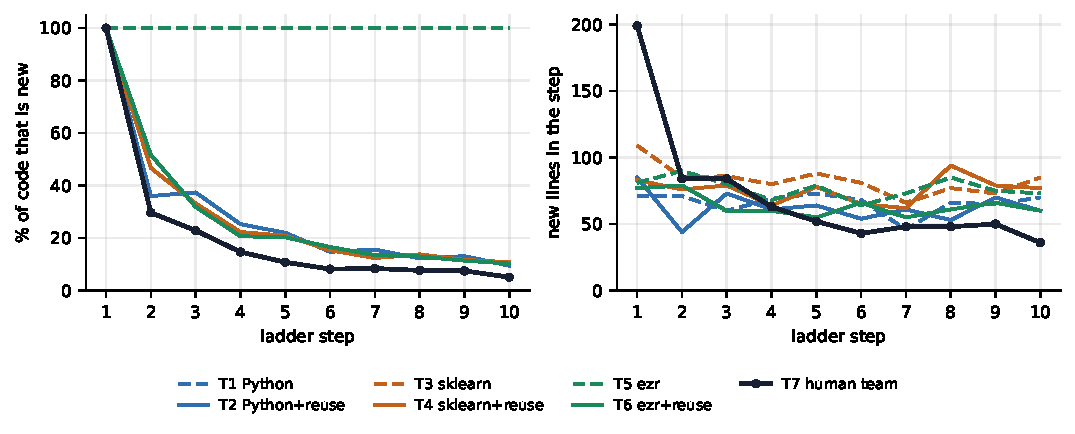
\includegraphics[width=\linewidth]{generated/fig_histograms.pdf}
\caption{Left: \% of the code that is new at each step. Right: new lines per step. Median over 9 ladders per LLM treatment; T7 is its x264 ladder. Solid lines reuse, dashed lines do not. Derived from the step tags.}\label{fig:hist}
\end{figure}

Table~\ref{tab:shrink} tests the falling-bars prediction with \same: it compares new lines in early steps (2--5) with late steps (7--10). For the LLM reuse arms, late steps are certified smaller in only 1 of 9 cells (T6 on Health). The other reuse cells are flat or larger, and T2 and T4 grow on x264. T7's x264 ladder shrinks (ratio 0.65). Some no-reuse arms also shrink slightly (T3 everywhere, T1 on x264 and NASA93, T5 on NASA93), so a shrink alone is not evidence of reuse.

\begin{table}[ht]
\caption{Median new lines in early (2--5) $\to$ late (7--10) steps, with the late/early ratio. $\downarrow$ = \same{} certifies late $<$ early; $=$ = indistinguishable; $\uparrow$ = certified larger.}\label{tab:shrink}
\footnotesize\begin{tabular}{llll}
\toprule
Treatment & x264 & NASA93 & Health \\
\midrule
T1 Python & 72$\to$62 (0.87) $\downarrow$ & 64$\to$62 (0.98) $\downarrow$ & 70$\to$64 (0.91) $=$ \\
T2 Python+reuse & 61$\to$68 (1.11) $\uparrow$ & 60$\to$58 (0.95) $=$ & 64$\to$60 (0.94) $=$ \\
T3 sklearn & 82$\to$74 (0.90) $\downarrow$ & 88$\to$78 (0.88) $\downarrow$ & 92$\to$76 (0.84) $\downarrow$ \\
T4 sklearn+reuse & 63$\to$68 (1.09) $\uparrow$ & 70$\to$89 (1.28) $=$ & 78$\to$86 (1.10) $=$ \\
T5 ezr & 78$\to$73 (0.94) $=$ & 78$\to$76 (0.97) $\downarrow$ & 78$\to$80 (1.02) $=$ \\
T6 ezr+reuse & 68$\to$72 (1.06) $=$ & 48$\to$52 (1.08) $=$ & 70$\to$57 (0.82) $\downarrow$ \\
T7 human team & 74$\to$48 (0.65) $\downarrow$ & 0$\to$0 (--) $=$ & 0$\to$0 (--) $=$ \\
\bottomrule
\end{tabular}
\end{table}

\subsection{Reuse versus no reuse}
Table~\ref{tab:reuse} compares each no-reuse arm with its reuse twin on the same background and dataset. Reuse writes \same-certified less code in \reuseCertified{} of 9 cells, and none of the 9 are certified larger. On x264 every pair ties. Per ladder, reuse saves about \savePython\% with plain Python (\totalPythonNoReuse{} $\to$ \totalPythonReuse{} lines), \savescikitlearn\% with scikit-learn (\totalscikitlearnNoReuse{} $\to$ \totalscikitlearnReuse) and \saveezr\% with ezr (\totalezrNoReuse{} $\to$ \totalezrReuse). The effects are small except for ezr on NASA93 and Health (Cliff's $\delta$ 0.90 and 0.49).

\begin{table}[ht]
\caption{Median new lines per step (steps 2--10, 27 steps per side), no reuse vs reuse, certified with \same.}\label{tab:reuse}
\footnotesize\begin{tabular}{llrrrl}
\toprule
Background & Dataset & No reuse & Reuse & Cliff's $\delta$ & \texttt{same} verdict \\
\midrule
Python & x264 & 68 & 61 & 0.04 & tie \\
Python & NASA93 & 64 & 60 & 0.23 & \textbf{reuse smaller} \\
Python & Health & 66 & 60 & 0.24 & \textbf{reuse smaller} \\
scikit-learn & x264 & 77 & 68 & 0.13 & tie \\
scikit-learn & NASA93 & 78 & 72 & 0.03 & tie \\
scikit-learn & Health & 85 & 79 & 0.04 & \textbf{reuse smaller} \\
ezr & x264 & 73 & 72 & 0.12 & tie \\
ezr & NASA93 & 77 & 50 & 0.90 & \textbf{reuse smaller} \\
ezr & Health & 77 & 58 & 0.49 & \textbf{reuse smaller} \\
\bottomrule
\end{tabular}
\end{table}

\subsection{Transfer across domains}
Only T7 carried code across domains (Figure~\ref{fig:transfer}). x264 needed \tSevenXtwo{} new lines. NASA93 then needed \tSevenNasa{} (\tSevenNasaShare\% of the codebase, one domain adapter) and Health \tSevenHealth{} (\tSevenHealthShare\%), with zero new lines for every later step. The LLM ladders cannot answer the transfer question, because the protocol restarted them in each domain.

\begin{figure}[ht]
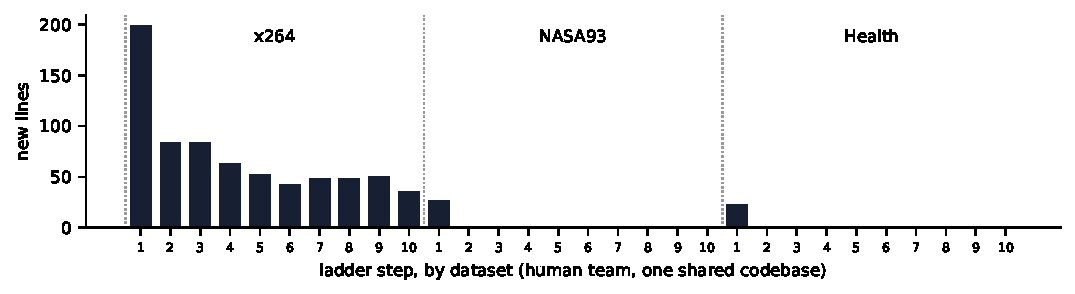
\includegraphics[width=\linewidth]{generated/fig_transfer.pdf}
\caption{Human team (T7): new lines per step across the three datasets, one shared codebase. Derived from the \texttt{t7/} tags.}\label{fig:transfer}
\end{figure}

\subsection{External metrics: is the code any good?}
Table~\ref{tab:guess} scores every treatment's guess code on the shared split. scikit-learn (T3, T4) predicts best: x264 error under half a second against 131\,s for guessing the average. ezr predicts worst: several of its models fall back to the training mean for unseen configurations. On NASA93's 19 test projects, T4--T7 are indistinguishable from guessing the average. Table~\ref{tab:race} scores race. On x264 with 10 evaluations, T3 ranks first and T7 second; T2 and T5 also beat random search. T4 and T6 tie with random search, and T1 ranks below it because one trial's tuner kept the slowest configurations. On Health, 13 of the 16 scorable LLM selectors (two trials recommend no configuration) read every recorded outcome and picked the minimum. That is a lookup, not a search, so we exclude them from comparison.

\begin{table}[ht]
\caption{Guess on the shared split: MAE and hit rate (median of trials), and rank by \same{} on per-row errors (0 = best).}\label{tab:guess}
\footnotesize\setlength\tabcolsep{3pt}\resizebox{\linewidth}{!}{\begin{tabular}{lrrrrrrrrr}
\toprule
 & \multicolumn{3}{c}{x264 (seconds)} & \multicolumn{3}{c}{NASA93 (effort)} & \multicolumn{3}{c}{Health (MRE)} \\
\cmidrule(lr){2-4}\cmidrule(lr){5-7}\cmidrule(lr){8-10}
Treatment & MAE & hit & rank & MAE & hit & rank & MAE & hit & rank \\
\midrule
T1 Python & 22.1 & 0.68 & 4 & 702 & 0.26 & \textbf{0} & 0.025 & 0.83 & 3 \\
T2 Python+reuse & 19.5 & 0.75 & 5 & 291 & 0.37 & \textbf{0} & 0.028 & 0.82 & 2 \\
T3 sklearn & 0.4 & 1.00 & \textbf{0} & 375 & 0.37 & \textbf{0} & 0.013 & 0.97 & \textbf{0} \\
T4 sklearn+reuse & 0.4 & 1.00 & 1 & 732 & 0.11 & 1 & 0.013 & 0.98 & 1 \\
T5 ezr & 24.3 & 0.67 & 3 & 837 & 0.11 & 1 & 0.093 & 0.32 & 4 \\
T6 ezr+reuse & 30.9 & 0.54 & 6 & 837 & 0.11 & 1 & 0.161 & 0.05 & 5 \\
T7 human team & 19.5 & 0.75 & 2 & 621 & 0.21 & 1 & 0.025 & 0.85 & 1 \\
\midrule Guess the average & 131 & -- & 7 & 673 & -- & 1 & 0.161 & -- & 6 \\
\bottomrule
\end{tabular}}
\end{table}

\begin{table}[ht]
\caption{Race. Regret: 0 = picked the best configuration, 1 = median. x264: same 200 unseen configurations, 10 evaluations (rank@20 with 20), seeds 1--10. $^*$Read every recorded result, a lookup rather than a search: not comparable.}\label{tab:race}
\footnotesize\setlength\tabcolsep{3pt}\resizebox{\linewidth}{!}{\begin{tabular}{lrrrrlr}
\toprule
 & \multicolumn{4}{c}{x264: tuner, 200 unseen configs} & \multicolumn{2}{c}{Health: selector} \\
\cmidrule(lr){2-5}\cmidrule(lr){6-7}
Treatment & regret & beats random & rank@10 & rank@20 & how it picked & regret \\
\midrule
T1 Python & 0.06 & 33\% & 4 & 4 & full history$^*$, held-out & 0.65 \\
T2 Python+reuse & 0.03 & 60\% & 2 & 1 & full history$^*$ & 0.04 \\
T3 sklearn & 0.00 & 80\% & 0 & 0 & held-out & 0.21 \\
T4 sklearn+reuse & 0.06 & 48\% & 3 & 2 & full history$^*$ & 0.00 \\
T5 ezr & 0.04 & 57\% & 2 & 1 & full history$^*$ & 0.00 \\
T6 ezr+reuse & 0.06 & 43\% & 3 & 2 & full history$^*$ & 0.00 \\
T7 human team & 0.01 & 50\% & 1 & 0 & budget 20 & 0.21 \\
\midrule Random search & 0.06 & -- & 3 & 3 & budget 20 & 0.29 \\
\bottomrule
\end{tabular}}
\end{table}

\subsection{Cost}
Table~\ref{tab:cost} gives the cost. Each arm used 46--71M tokens, over 90\% of them cached input because the agent rereads the code every turn. In total the six arms took \hoursRuns{} hours of LLM time and about \$\costRuns{} at API list prices. The setup and planning chat cost another \$\costSetup, for about \$\costAll{} against a \$100-per-person budget. The marginal spend was covered by ChatGPT Plus subscriptions; we never exceeded the budget. T1--T3 figures come from a teammate's archived sessions, which overlap in places, so treat them as upper bounds.

\begin{table}[ht]
\caption{Cost per treatment over 9 ladders (Codex logs; \texttt{results/cost.csv}).}\label{tab:cost}
\footnotesize\begin{tabular}{lrrrr}
\toprule
Treatment & tokens & cached & LLM hours & \$ at API prices \\
\midrule
T1 Python & 46M & 95\% & 1.1 & \$2.03 \\
T2 Python+reuse & 71M & 95\% & 1.4 & \$2.84 \\
T3 sklearn & 67M & 96\% & 1.5 & \$2.62 \\
T4 sklearn+reuse & 55M & 95\% & 3.5 & \$8.83 \\
T5 ezr & 46M & 95\% & 2.2 & \$2.26 \\
T6 ezr+reuse & 47M & 94\% & 2.1 & \$2.23 \\
\midrule All six LLM arms & 332M & & 11.7 & \$20.81 \\
Setup and planning chat & 262M & & 3.0 & \$40.04 \\
\bottomrule
\end{tabular}
\end{table}

%% ============================================================
\section{Discussion}\label{sec:discussion}

\paragraph{Verdict per domain.}
\emph{x264:} the rival wins for LLMs. No pair shows a certified reuse saving, and the reuse arms' late steps are no smaller than their early steps. The human ladder shrinks (0.65).
\emph{NASA93:} reuse saves code for Python and ezr, but no reuse arm shrinks along the ladder, so the result is mixed. The human core transferred for \tSevenNasa{} lines.
\emph{Health:} reuse saves code for all three backgrounds, but only T6 shrinks (1 of 3 reuse arms), so this is mixed and leans rival on shrinking. The human core transferred for \tSevenHealth{} lines.

\paragraph{Overall.} For LLM ladders the rival holds on the central prediction: new code per step stays flat, and the falling share is an artefact of a growing denominator. Reuse instructions buy a modest, partly certified saving (\reuseCertified{} of 9 cells, \savePython--\saveezr\% per ladder), but not cheaper tokens or dollars. Prediction quality follows the library (scikit-learn), not reuse. The Timm pattern appears only for the human team: a falling curve and near-free transfer. That evidence rests on one run per domain, and its early-vs-late test uses only four steps a side.

\paragraph{Internal versus external.} Internal metrics alone would have picked the wrong winner. T6 (ezr + reuse) writes the least LLM code but is the worst predictor, while T3 writes the most and predicts best.

\paragraph{Honest failures.}
\begin{itemize}
\item \emph{N=3} trials per LLM arm, and one for T7.
\item \emph{Reconstructed tags.} The step history was rebuilt from snapshots, not committed live.
\item \emph{No ezr tuning.}
\item \emph{One invalid run.} One race (T1 trial~1, x264) used 56 evaluations against the baseline's 32; it is kept and flagged.
\item \emph{Self-reported metrics.} T1/T3 LOC were inflated, error counts were counted differently by each arm, and one step logged 8,744 new lines.
\item \emph{Model drift.} T4 trial~1 ran on a different model.
\item \emph{Long prompts.} Prompts were specifications, not one-line requirements.
\item \emph{Selectors that read the answers.} Health race selectors read every recorded result.
\item \emph{An earlier claim we correct.} Our task talk reported a 30--40\% reuse saving from the self-reported counts; the tag-derived figures here replace it.
\end{itemize}
With more budget we would run 10 trials per arm on one pinned model, give the LLM arms cross-domain carry-over, and tune ezr.

%% ============================================================
\section*{AI Disclosure}
\paragraph{What AI wrote.} All T1--T6 code, tests and per-step metrics were written by the Codex agent (gpt-5.6-luna; T4 trial~1 on gpt-6.1-sol). T7 was written by the team.
%% TODO: state any AI assistance used for T7.
The evaluation harness, the tag reconstruction and histogram scripts, this report's figure and table scripts, and a first draft of this text were written with Claude Code (Claude Opus 5.5) and reviewed by the team.

\paragraph{LLM errors we caught.}
\begin{itemize}
\item A tuner that sorted the wrong way and kept the slowest x264 configurations (T1 trial~3).
\item A linear model with no intercept that predicts negative times (T6 trial~1; MAE 456\,s).
\item ``Predictors'' that are lookup tables returning the mean for unseen inputs (T2, T5, T6).
\item Selectors that read every answer (Health, T2/T4/T5/T6).
\item An unequal-budget race comparison (T1 trial~1).
\item An 8,744-line LOC entry.
\item LOC over-reported about 1.5$\times$ (T1, T3).
\end{itemize}

\paragraph{Errors in AI-assisted analysis we caught.}
\begin{itemize}
\item A token estimate from saved text that was about 200$\times$ too low.
\item A teammate's archive script whose first pass over-counted tokens about 5$\times$ and gave impossible medians.
\item A cost-total arithmetic slip.
\item Scoring adapters that read the wrong output field. Each was checked against the program's own log.
\end{itemize}
Details: \texttt{docs/ai\_disclosure.md}.

\bibliographystyle{ACM-Reference-Format}
\bibliography{references}

\end{document}
